% !TeX spellcheck = de_DE
\chapter{Grundlagen}

S/MIME ist standardisiertes Format zur Verschlüsselung von E-Mails und setzt X.509 Zertifikate ein. S/MIME und OpenPGP sind inkompatibel (Absatz vgl. \cite[S. 667f]{book:kryptoschmeh}).


\vref{fig:alice-bob-mallory} zeigt die beschriebenen drei bzw. vier Akteure der Kommunikation.

\begin{minipage}[c]{\textwidth}
	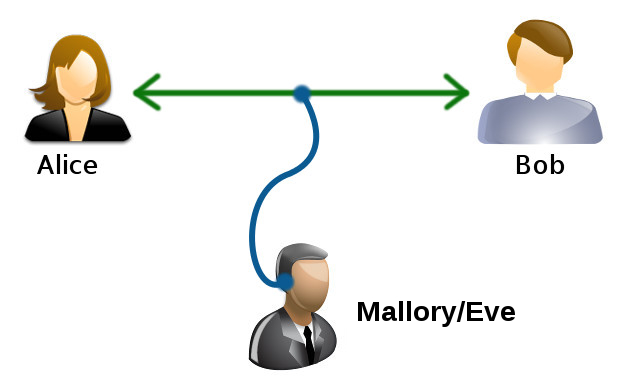
\includegraphics{res/Alice-bob-eve}
	\figcaption[Vorstellung von Alice, Bob und Mallory/Eve]{\mbox{Vorstellung von Alice, Bob und Eve}\\
		\footnotesize{Quelle: Ursprünglich von Didia (Own work) [CC BY-SA 4.0 (http://creativecommons.org/licenses/by-sa/4.0)], via Wikimedia Commons mit Änderung des Bezeichnung Mallory \cite{alicebobeve}}}
	\label{fig:alice-bob-mallory}
\end{minipage}


\section{OpenPGP}\label{openpgp}
\begin{formal}
	Cite mit Seitenangabe
\end{formal}
Es ist eines der am weitesten verbreiteten Werkzeuge zur E-Mail- und Dateiverschlüsselung~(\cite[S. 995]{book:cyclocryptosec}).

\begin{formal}
	Cite eines RFC
\end{formal}
1998 standardisierte die OpenPGP Working Group PGP bei der \gls{IETF} als "`OpenPGP Message Format"' in \cite{rfc4880}.

\begin{formal}
	vref,  smartref und autoref im Vergleich
\end{formal}

\textbf{\vref{loesung}}\\ 
\textbf{\smartref{loesung}}\\
\autoref{loesung}


\begin{formal}
	cite mit mehreren Quellen 
\end{formal}
\cite{heise-10jahrepgp, heise-gpgsupport, gpg-nytfounding, license-gpg})


\begin{formal}
	benutzung von verb
\end{formal}
In der vorliegenden Arbeit wird diese Software für Untersuchungen und zu Demonstationszwecken in den Versionen \verb|gpg 1.4.18| bzw. \verb|gpg2 2.0.28| verwendet



\begin{formal}
	Eine Referenz auf eine Zeile in einem Listing
\end{formal}
Die verwendeten Subpaket-Klassen beschränken sich lediglich auf 2 (Datum) und 29 (Grund des Widerrufs) in Zeile \ref{code:hashed-subpkt-2}f.

\begin{minipage}[t]{\textwidth}
	\begin{lstlisting}[language=bash,label={lst:pgp-packet},deletekeywords={test},caption={Ein PGP-Paket}]
:signature packet: algo 1, keyid 959FEB541D9FCFE5
version 4, created 1462880534, md5len 0, sigclass 0x30
digest algo 2, begin of digest b3 50
hashed subpkt 2 len 4 (sig created 2016-05-10)(*\label{code:hashed-subpkt-2}*)
hashed subpkt 29 len 15 (revocation reason 0x00 (this is a test))
subpkt 16 len 8 (issuer key ID 959FEB541D9FCFE5)
data: [2046 bits]
	\end{lstlisting}
\end{minipage}


\begin{formal}
	Eine in der Breite beschränkte Grafik (0.8)
\end{formal}

\begin{center}
\begin{minipage}[c]{0.8\textwidth}
	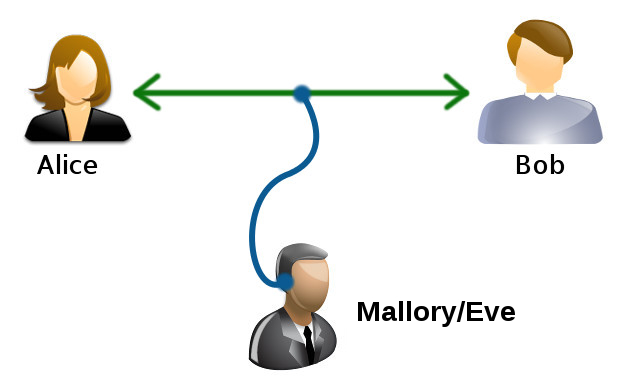
\includegraphics{res/Alice-bob-eve}
  \figcaption[Vorstellung von Alice, Bob und Mallory/Eve]{\mbox{Vorstellung von Alice, Bob und Eve}\\
	\footnotesize{Quelle: Ursprünglich von Didia (Own work) [CC BY-SA 4.0 (http://creativecommons.org/licenses/by-sa/4.0)], via Wikimedia Commons mit Änderung des Bezeichnung Mallory \cite{alicebobeve}}}
	\label{alicebob-2}
\end{minipage}
\end{center}


\begin{formal}
	Eine in der Höhe beschränkte Grafik (0.6); \textbf{Zeigen wie man subscripts in Captions unterbringt}
\end{formal}
\begin{figure}[h!]
	\centering
	\Oldincludegraphics[height=0.60\textheight]{res/Alice-bob-eve}
     \caption[Subscript in caption]{Subscript test \mbox{$Variable_{\textnormal{subscript}}$}\\
	\footnotesize{Quelle: Ursprünglich von Didia (Own work) [CC BY-SA 4.0 (http://creativecommons.org/licenses/by-sa/4.0)], via Wikimedia Commons mit Änderung des Bezeichnung Mallory \cite{alicebobeve}}}
	\label{key-upload-flowchart-section}
\end{figure}
\clearpage

\begin{formal}
	Eingerückter Text
\end{formal}

\begin{adjustwidth}{1em}{0em}

% Ja, das darf kein Paragraph sein, weil sonst die EInrückung nicht funktioniert
\keyword{1. Sitzungs-ID} 
Lorem ipsum dolor sit amet

\paragraph{2. Authentifizierung}
Lorem ipsum dolor sit amet

\paragraph{3. Verifikation}
Lorem ipsum dolor sit amet

\end{adjustwidth}


Ein Beispielaufruf des Uploads zeigt \vref{lst:ra-rest-cert-demo}.

\begin{formal}
	Inlining von Latex-Kommandos in Listings (z.B. zum Fett-drucken) (escapeinside)
\end{formal}
\begin{minipage}[t]{\textwidth}
	\begin{lstlisting}[label={lst:ra-rest-cert-demo},caption={Beispielanfrage zum Upload eines Keys},escapeinside={(\%}{\%)}]
(%\textbf{POST}%) (%\url{/certs/?pid=flJvlYAH...CKQZusIT&cert_type=encr}%) HTTP/1.1
[...]
(%\fbox{--01ead4a5-7a67-4703-ad02-589886e00923}%)
[...]
--01ead4a5-7a67-4703-ad02-589886e00923
	\end{lstlisting}
\end{minipage}